\documentclass[tikz,border=25pt]{standalone}
\usepackage{tikz}
\usepackage{lmodern}
\usetikzlibrary{shapes.geometric, arrows.meta, positioning, fit, calc, backgrounds}

% Premium Dark Theme Colors
\definecolor{cBg}{HTML}{0D1117} 
\definecolor{cItemBg}{HTML}{21262D}
\definecolor{cItemBorder}{HTML}{30363D}

\definecolor{cText}{HTML}{FFFFFF}
\definecolor{cTextMuted}{HTML}{8B949E}

\definecolor{cServerAccent}{HTML}{58A6FF} % Bright Blue
\definecolor{cNetworkAccent}{HTML}{3FB950} % Bright Green
\definecolor{cClientAccent}{HTML}{E3B341} % Bright Yellow

\definecolor{cGladBg}{HTML}{1F6FEB}
\definecolor{cGladText}{HTML}{FFFFFF}

\definecolor{cOnlineBg}{HTML}{04260F}
\definecolor{cOnlineBorder}{HTML}{1A7F37}
\definecolor{cOnlineText}{HTML}{3FB950}

\definecolor{cArrow}{HTML}{8B949E}

\begin{document}
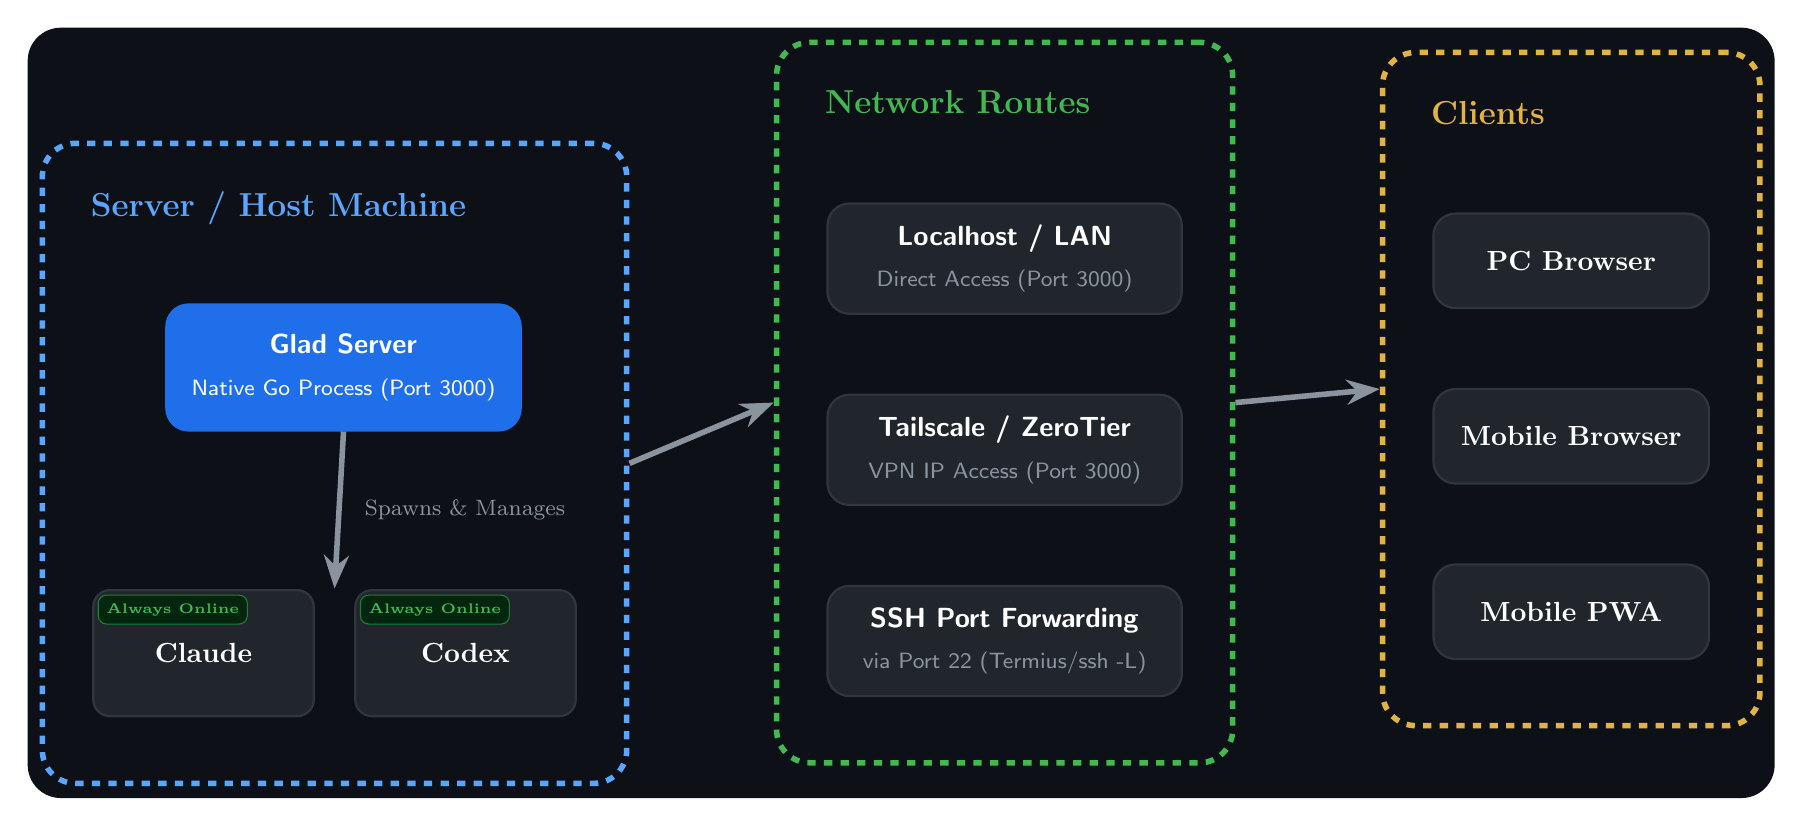
\begin{tikzpicture}[
    font=\sffamily\color{cText},
    >=Stealth,
    background rectangle/.style={fill=cBg, rounded corners=12pt},
    show background rectangle,
    % Core item styles
    box/.style={rectangle, rounded corners=8pt, draw=cItemBorder, thick, fill=cItemBg, minimum height=1.4cm, minimum width=4.5cm, align=center},
    glad_box/.style={rectangle, rounded corners=8pt, draw=cGladBg, thick, fill=cGladBg, text=cGladText, minimum height=1.6cm, minimum width=4.5cm, align=center},
    simple_box/.style={rectangle, rounded corners=8pt, draw=cItemBorder, thick, fill=cItemBg, minimum height=1.2cm, minimum width=3.5cm, align=center, font=\bfseries\color{cText}},
    session_box/.style={rectangle, rounded corners=6pt, draw=cItemBorder, thick, fill=cItemBg, minimum height=1.6cm, minimum width=2.8cm, align=center, font=\bfseries\color{cText}},
    always_online_label/.style={rectangle, rounded corners=3pt, draw=cOnlineBorder, fill=cOnlineBg, text=cOnlineText, font=\tiny\bfseries, inner sep=3pt},
    % Wrapper styles - Transparent (no fill) to avoid rendering issues, drawn explicitly
    wrapper/.style={rectangle, rounded corners=12pt, dashed, draw, line width=2pt, inner sep=18pt},
    server_wrapper/.style={wrapper, draw=cServerAccent},
    network_wrapper/.style={wrapper, draw=cNetworkAccent},
    client_wrapper/.style={wrapper, draw=cClientAccent},
    % Arrow style
    arrow/.style={->, line width=2pt, color=cArrow}
]

% --- SERVER NODE ---
\node[glad_box] (glad) {\textbf{Glad Server}\\[3pt] \footnotesize\color{cText} Native Go Process (Port 3000)};

% Sessions
\node[session_box, below=2cm of glad, xshift=1.55cm] (s2) {Codex};
\node[session_box, left=0.5cm of s2] (s1) {Claude};

\foreach \n in {s1, s2} {
    \node[always_online_label, anchor=north west, xshift=2pt, yshift=-2pt] at (\n.north west) {Always Online};
}

\node[fit=(s1)(s2), inner sep=0pt] (sessions) {};

\draw[arrow] (glad.south) -- node[right, font=\footnotesize\color{cTextMuted}, align=center, xshift=5pt] {Spawns \& Manages} (sessions.north);

% Server Wrapper (Stretching top with a dummy coordinate to fit the title)
\coordinate (server_top) at ([yshift=1.4cm]glad.north);
\coordinate (server_bottom) at ([yshift=-0.2cm]sessions.south);
\node[server_wrapper, fit=(server_top)(server_bottom)(s1)(s2)] (server) {};
\node[anchor=north west, font=\large\bfseries\color{cServerAccent}, xshift=15pt, yshift=-15pt] at (server.north west) {Server / Host Machine};


% --- NETWORK NODE ---
\node[box, right=2.5cm of server, yshift=2.6cm] (local) {\textbf{Localhost / LAN}\\[3pt] \footnotesize\color{cTextMuted} Direct Access (Port 3000)};
\node[box, below=1cm of local] (vpn) {\textbf{Tailscale / ZeroTier}\\[3pt] \footnotesize\color{cTextMuted} VPN IP Access (Port 3000)};
\node[box, below=1cm of vpn] (ssh) {\textbf{SSH Port Forwarding}\\[3pt] \footnotesize\color{cTextMuted} via Port 22 (Termius/ssh -L)};

% Network Wrapper
\coordinate (network_top) at ([yshift=1.4cm]local.north);
\coordinate (network_bottom) at ([yshift=-0.2cm]ssh.south);
\node[network_wrapper, fit=(network_top)(network_bottom)(local)(vpn)(ssh)] (network) {};
\node[anchor=north west, font=\large\bfseries\color{cNetworkAccent}, xshift=15pt, yshift=-15pt] at (network.north west) {Network Routes};


% --- CLIENTS NODE ---
\node[simple_box, right=2.5cm of network, yshift=1.8cm] (pc) {PC Browser};
\node[simple_box, below=1cm of pc] (mobile) {Mobile Browser};
\node[simple_box, below=1cm of mobile] (pwa) {Mobile PWA};

% Clients Wrapper
\coordinate (clients_top) at ([yshift=1.4cm]pc.north);
\coordinate (clients_bottom) at ([yshift=-0.2cm]pwa.south);
\node[client_wrapper, fit=(clients_top)(clients_bottom)(pc)(mobile)(pwa)] (clients) {};
\node[anchor=north west, font=\large\bfseries\color{cClientAccent}, xshift=15pt, yshift=-15pt] at (clients.north west) {Clients};


% --- ARROWS ---
\draw[<->, arrow] (server.east) -- (network.west);
\draw[<->, arrow] (network.east) -- (clients.west);

\end{tikzpicture}
\end{document}
